\documentclass[a4paper,12pt,twoside]{report}
\usepackage{a4wide}
\usepackage{hyperref}
\usepackage{color}
\usepackage{pgfplots}
\usepackage[final]{pdfpages}

\usepackage{graphicx}
\graphicspath{ {images/}}
\usepackage{float}

\usepackage{fancyhdr}
\pagestyle{fancy} %TODO: Headers need work

\parindent 0pt
\parskip 6pt

\begin{document}

%%%%%%%%%%%%%%%%%%%%%%%%%%%%%%%%%%%%%%%%%%%%%
% Macros
\newcommand{\todo}[1]{{\color{red} TODO: {#1}}}
\newcommand{\imageplaceholder}[3][Placeholder Image]{
  \begin{figure}[H]
    \centering
    
\includegraphics[width=#2,height=#3]{pixel.png}
    \caption{#1}
  \end{figure}
}

\begin{titlepage}
%%%%%%%%%%%%%%%%%%%%%%%%%%%%%%%%%%%%%%%%%%%%%%
% Title Page

\newcommand{\HRule}{\rule{\linewidth}{0.5mm}} % Defines a new command for the horizontal lines, change thickness here

\center % Center everything on the page
 
%----------------------------------------------------------------------------------------
%	HEADING SECTIONS
%----------------------------------------------------------------------------------------

\textsc{\LARGE University of Cambridge}\\[1.5cm] % Name of your university/college
\textsc{\Large Computer Science Tripos}\\[0.5cm] % Major heading such as course name
\textsc{\large Part II Project}\\[0.5cm] % Minor heading such as course title

%----------------------------------------------------------------------------------------
%	TITLE SECTION
%----------------------------------------------------------------------------------------

\HRule \\[0.4cm]
{ \huge \bfseries Time-Lapse Based Weather Classification}\\[0.0cm] % Title of your document
\HRule \\[1.5cm]
 
%----------------------------------------------------------------------------------------
%	AUTHOR SECTION
%----------------------------------------------------------------------------------------

\begin{minipage}{0.4\textwidth}
\begin{flushleft} \large
\emph{Author:}\\
Roman \textsc{Kolacz} % Your name
\end{flushleft}
\end{minipage}
~
\begin{minipage}{0.4\textwidth}
\begin{flushright} \large
\emph{Supervisor:} \\
Advait \textsc{Sarka} % Supervisor's Name
\end{flushright}
\end{minipage}\\[2cm]

% If you don't want a supervisor, uncomment the two lines below and remove the section above
%\Large \emph{Author:}\\
%John \textsc{Smith}\\[3cm] % Your name

%----------------------------------------------------------------------------------------
%	DATE SECTION
%----------------------------------------------------------------------------------------

{\large \today}\\[3cm] % Date, change the \today to a set date if you want to be precise

%----------------------------------------------------------------------------------------
%	LOGO SECTION
%----------------------------------------------------------------------------------------


\includegraphics[height=4cm]{pixel.png}\\
A logo/image/something cool
 
%----------------------------------------------------------------------------------------

\vfill % Fill the rest of the page with whitespace

\end{titlepage}

\chapter*{Proforma}
%%%%%%%%%%%%%%%%%%%%%%%%%%%%%%%%%%%%%%%%%%%%%%
% Proforma, table of contents, list of figures

\begin{tabular}{ll}
  \bf Name: & Roman Kolacz \\
  \bf College: & Downing College \\
  \bf Project Title: & TIme-Lapse Based Weather Classification \\
  \bf Examination: & Computer Science Tripos - Part II \\
  \bf Word Count: \\
  \bf Project Originator: & Alan Blackwell \\
  \bf Project Supervisor: & Advait Sarkar \\
\end{tabular}

\section*{Initial Project Aims}
The initial aim of the project was to associate time-lapse video with external data sources by using a time-lapse video of an outside location to tell the weather. This would then be evaluated against real weather information and demonstrated graphically.

\section*{Work Completed}
Over a months worth of data has been gathered and a classifier has been built which uses extracted image metrics and actual weather data to train a machine learning classifier which can then infer the weather.
The accuracy of several machine learning algorithms has been tested and the best for each data set has been used to maximise overall accuracy. 
The initial plan was changed from using manually hard-coded rules for weather classification to using machine learning to do so instead.

\section*{Special Difficulties}
None.
\section*{Decleration of Originality}
I, Roman Kolacz of Downing College, being a candidate for Part II of the Computer Science Tripos, hereby declare that this disseration and the work described in it are my own work, unaided except as may be specified below, and that the disseration does not contain material that has aready been used to any substantial extent for a comparable purpose.

\bigskip
\leftline{\bf Signed:}

\bigskip
\leftline\bf{\bf Date:}

\newpage

\section*{Acknowledgements}
Advait 
Alan 
\todo{More detail here} 

\tableofcontents

\listoffigures

%%%%%%%%%%%%%%%%%%%%%%%%%%%%%%%%%%%%%%%%%%%%%%
% Dissertation content
\chapter{Introduction}

\section{Aims}

\section{Challenges}

\section{Related Work} %Literature Review

\chapter{Preparation}

\section{Requirements Analysis}


\section{Data Gathering}
A Raspberry Pi\cite{x} with the Camera Module\cite{x} was used to take pictures at a 5 minute interval out of my window overlooking the Downing College court.

\imageplaceholder[A picture of the Raspberry Pi and Camera setup]{12cm}{8cm}

At each interval, a new line would be added to a csv file which would contain the necessary image metrics to train the classifier as well as actual weather data and basic information such as the name of the corresponding file, the time, date, etc.

\imageplaceholder[An example picture taken from the setup]{12cm}{8cm}


Raspberry pi, camera, forecast, etc

\section{Time Lapse}
Time lapse is a relatively unexplored way of compressing events which occur over extended periods of time into smaller, more managable videos. 

\section{Machine Learning}
A large amount of research was devoted towards learning how different machine learning algorithms can be used and which would excel in different parts of the weather classification system.

\subsection{Random Forest}
A decision tree in machine learning is a tree used to reach a conclusion based on given parameters. At each branch, a path is chosen based on a condition, and the tree is traversed in this way until a leaf is reached with an outcome. 

Decision trees are incredibly simple to generate and use, though have a very high variance with results (even small changes in inputs can cause drastically different branch paths to drastically different results) as well as a tendency to overfit data (so outliers are significantly accounted for and general patterns are not formed), and are thus not usable as a reliable machine learning algortihm without modifications.

\imageplaceholder[An example decision tree for classifying the weather]{8cm}{14cm}

A random forest is a machine learning algorithm which builds upon decision trees and corrects for their variance and tendency to overfit. They work by using a random set of decision trees which individually classify the data- then either the mode or the mean of the results is used as the final outcome.

\imageplaceholder[Random Forest Graph of some sort]{8cm}{6cm}

Random forests run relatively accurately and also incredibly quickly and so were used from an early stage in the project to see if classification was working, and to give a rough estimate of the overall accuracy of classification (primarily to see if it was better than randomly guessing the weather).

\subsection{Multilayer Perceptron}
A single perceptron simply returns a 0 or 1 based on a given imput and a given activation function based on the input. It aims to divide the data into two sets and so the number returned determines which side of the division the given value should lie.

A single layer perceptron recursively trains itself and adjusts weightings of the output of each of the perceptrons within the layer on each recursion to improve the overall outcome of the classification (of the training set).

A multilayer perceptron uses multiple layers of perceptrons, including various hidden layers between the input and output layers.

\subsection{J48}
J48 is an open source implementation of the C4.5 algorithm which also uses a decision tree to build a classifier. At each node in the tree, the algorithm chooses the attribute which most effectly splits the set of training samples into consistent subsets. This, done recursively eventually forms the complete tree.


\section{Choice of Tools}
\subsection{Programming Language}
I used Java for the entirety of the project. This was chosen to ease development accross different operating systems, to be able to use the WEKA library (which my supervisor was very familiar with), and from sheer familiarity and simplicity of the language. 
Performance wasn't an issue as the classifying was done in a single run whenever results were required. 

\subsection{Libraries}
\subsubsection{WEKA}
The WEKA\cite{x} library was used for the machine learning portion of the project. It provides the functionality to train it's many included classifiers on CSV files with whatever options need to be set. 

Some problems arose with training the classifiers to use a mixed data set (continious and discrete) which only existed in the newer versions of WEKA, so older versions were used until a workaround was found \todo{what was the workaround}.

\subsubsection{Forecast.io}
The Forecast.io\cite{x} API was used for gathering the real weather data. It provides an incredibly accurate forecast based on longitude and latitide for all the data which was required, and more.Forecast.io allows 1000 free queries daily, which is well above the amount required for the 5-minutely querying of my project.

The foreast.io API takes a longitude and latitude and returns JSON file with detailed weather information subdivided into minutely, hourly and daily; each of which contain data for several \todo{how many?} units of time in either direction. I used a wrapper\cite{x} library to deserialize the JSON format into classes with the relevant data.

\subsection{Backups}
Dropbox\cite{x} and github\cite{x} were both used to ensure the project was safe should my hard drive become inaccessible for whatever reason. 
This was done by creating the git repository within a dropbox folder. Versioning and branching wasn't used due to the linear nature of the project and the fact that the work was done by a single person on a single computer at a time.

\chapter{Implementation}
\imageplaceholder[Processing Pipeline]{8cm}{6cm}

\section{Gathering Image Data}

\subsection{Feature Extraction}
Once images had been obtained with the hardware detailed above, image features had to be extracted in order to train the classifier with. Initially OpenCV\cite{x} was going to be used, though soon into development, there was a realisation that there was little need for it.

The features extracted include:
\begin{itemize}
  \item Average Hue
  \item Brightness Histogram
  \item Each of RGB histograms
\end{itemize}

These were obtained by sampling each pixel in the images using the java BufferedImage\cite{x} class' ability to return the RGB vales of the pixels of an image in sequence as an array of bytes.
The brightnss value of a set of RGB values was determined by the luminance function\cite{x}.
$$Y = 0.2126R + 0.7152G + 0.0722B$$
where Y is the luminance and R, G and B are Red, Green and Blue respectively.

The histograms are a size 256 array containg the number of pixels with the given RGBY value.

The average hue was obtained by simply averaging the RGB values of each of the pixels in each image.

\section{Data Storing}
Comma-Separated Value (csv) files were used to store the data in a convenient way for both anyone reading the data and for the WEKA library. The data stored included the name of the image, the time and date it was taken, as well as the actual weather information occuring in the image and the features extracted to train a classifier. Blank columns were left for the predicted weather information which would be filled in by the classifier once it was trained and ran.

\section{Machine Learning}
Once the features and real weather data had been stored in a csv file, the machine learning aspect of the project could begin. The data was split into training and testing with an 80:20 split such that 80\% of the data was used to train a classifier and the remaining 20\% was then used to evaluate the trained classifier. The data was split randomly, and placed into two seperate csv files.

The irrelevant columns (such as the name/date/etc) in the csv files then had to be filtered so that they were not used in the training of the classifier to not allow training using data which wasn't extracted from the images themselves.
 
\section{Sanity Checking}
Sanity checking ensures that everything is going well, and if it isn't, that a user responsible is made aware sooner rather than later to fix whatever problems may have arisen.

A sanity check which was employed in this project involved making sure that the Raspberry Pi was taking images and uploading them to dropbox continiously, as a large set of data was an integral part of the success of this project.

\todo{This section is a bit pointless\ldots Remove?}

\chapter{Evaluation}

\section{Cross Validation}
Cross validation is a technique used to evaluate machine learning algorithms by testing them on 100\% of the data set. In this case, the data was split into training:testing with an 80:20 ratio. This was done five times such that each of the testing splits were unique and formed the complete data set, so each point of data was used to train four classifiers and was tested by one (which it didn't train).

It is important not to train and test machine learning classifiers using the same data, as classifiers which don't learn (and rather, remember) would perform extraordinarily well.

\section{Description of Data}
The input data had to be analysed and described to give meaning to the evaluation. 

\subsection{Icon}
\imageplaceholder[Icon data bar chart]{10cm}{6cm}
There were initial concerns with how varied the icon would be given the high likelihood of cloudy weather in the UK, especially during the period of data gathering. Fortunately, forecast.io distinguishes between cloudy and partly cloudy, with the latter being further distinguised into day and night classes. Due to this, the data is relatively spread out and a highly accurate classifier would not be able to be built by simply guessing cloudy all the time, as per the initial concerns.

\subsection{Cloud Cover}
\imageplaceholder[Some Graph for Cloud Cover]{10cm}{6cm}
As the graph above shows, the cloud cover is distribted qute uniformly between 0 (no cloud cover) and 1 (complete cloud cover), with the mean and median being almost equal. The standard deviation is 31\% cloud cover, so the classifier should aim to classify within that percentage.

\subsection{Precipitation}
\imageplaceholder[Some Graph for Precipitation]{10cm}{6cm}
Much unlike the cloud cover, the precipitation is massively skewed toward the lower 10th percentile, which indicates that there was generally very little rain in the data gathering stage of the project.
Deviation of 23\%.

\subsection{Temperature}
\imageplaceholder[Some graph for Temperature]{10cm}{6cm}
The temperature is somewhat better distributed than the precipitation, though not as uniformly as the cloud cover. The data was gathered over the winter and early spring months, and so the temperature is generally very low with later dates having the higher temperatures. This would likely be a more uniform distribution if the data was to be taken over a longer period of time encompassing at least all four seasons.

Deviation of 2.9 degrees.

\section{Analysis of Classifiers}
The discrete data was analysed by simply comparing the percentage of correct classifications for each class.
The continious data was analysed by calculating the root-mean-square error, given by
$$RMSD = \sqrt{\frac{\sum_{t=1}^n (x_t - y_t)^2}{n}}$$
where x is the actual value and y is the predicted value in each line of data.

\subsection{Random Forest}
Random forests were analysed with a varying number of trees ranging from 1 to 100, and then 200. Results wer otained with each of the number of trees to analyse how performance changes for different classes with the increase in trees.

\subsubsection{Icon}
\imageplaceholder[Icon graph per number of trees]{10cm}{6cm}
The accuracy of the classifier for icon increased with the number of trees up to about 55-56\% at 50 trees. There was negligable increase in accuracy after this point, suggesting that the classifier has reached its potential for the feature set.

56\% as an accuracy is rather good- well above randomly guessing and well above the mode value percentage. 

\subsubsection{Sunrise and Sunset}
\imageplaceholder[Icon graph per number of trees]{10cm}{6cm}


\subsubsection{Cloud Cover}
\imageplaceholder[Icon graph per number of trees]{10cm}{6cm}

\subsubsection{Precipitation}
\imageplaceholder[Icon graph per number of trees]{10cm}{6cm}

\subsubsection{Temperature}
\imageplaceholder[Icon graph per number of trees]{10cm}{6cm}

\subsection{J48}
16\% accuracy on icon and nothing else becuase it only works on discrete data.

\subsection{Multilayer Perceptron}

\subsubsection{Icon}
The multilayer perceptron had a 36.1\% accuracy rate with classifying the icon. This is marginally better than assigning the mode result to every instance, and also better than the average case of randomly assigning icons. However, this is by no means a reliable classifier for classifying the icon as 36\% is a generally low success rate for classification (it's wrong more often than it's right). Other options will have to be explored.

\subsubsection{Sunrise and Sunset}
The sunrise and sunset had a root-mean-square error of 8:12 and 5:11 minutes respectively.
\todo{data descriptor for this}

\subsubsection{Cloud Cover}
The multilayer perception had a 35\% root-mean-square error for cloud cover, which is outside of the 31\% standard deviation, though only just. Being within two standard deviations, it's still a somewhat accurate way of deducing cloud cover, though not ideal.

\subsubsection{Precipitation}
The precipitation predictions had a root-mean-square error of 33\%, which is well outside of the stanard deviation of 23\%. 

\subsubsection{Temperature}
The multilayer perceptron had a 1.6 degree root-mean-square error when telling the temperature, which is well within a standard deviation of 2.9 degrees. This is an excellent result and is unlikely to be beaten by the performance of any other classifiers.

\subsubsection{Summary}
Overall the Multilayer Perceptron is a rather inaccurate classification algorithm in all cases with the exception of the rather surprisingly accurate temperature reading.

\section{Overall Results}
Summary of overall results/accuracy, etc?

See which pair of in/out was the most and least successful with classification.
Maybe pictures of which were the most innacurate??

\chapter{Conclusions}

\section{Future Work}
Extensions, etc?
- More classifiers
- Better feature extraction- perhaps a histogram for each segment in the image (divide into 9 or something)

\section{Changes}
Could be merged with above?

\addcontentsline{toc}{chapter}{Bibliography}
\bibliographystyle{plain}
\bibliography{refs}{}

\chapter{Appendices}


%%%%%%%%%%%%%%%%%%%%%%%%%%%%%%%%%%%%%%%%%%%
% Project Proposal
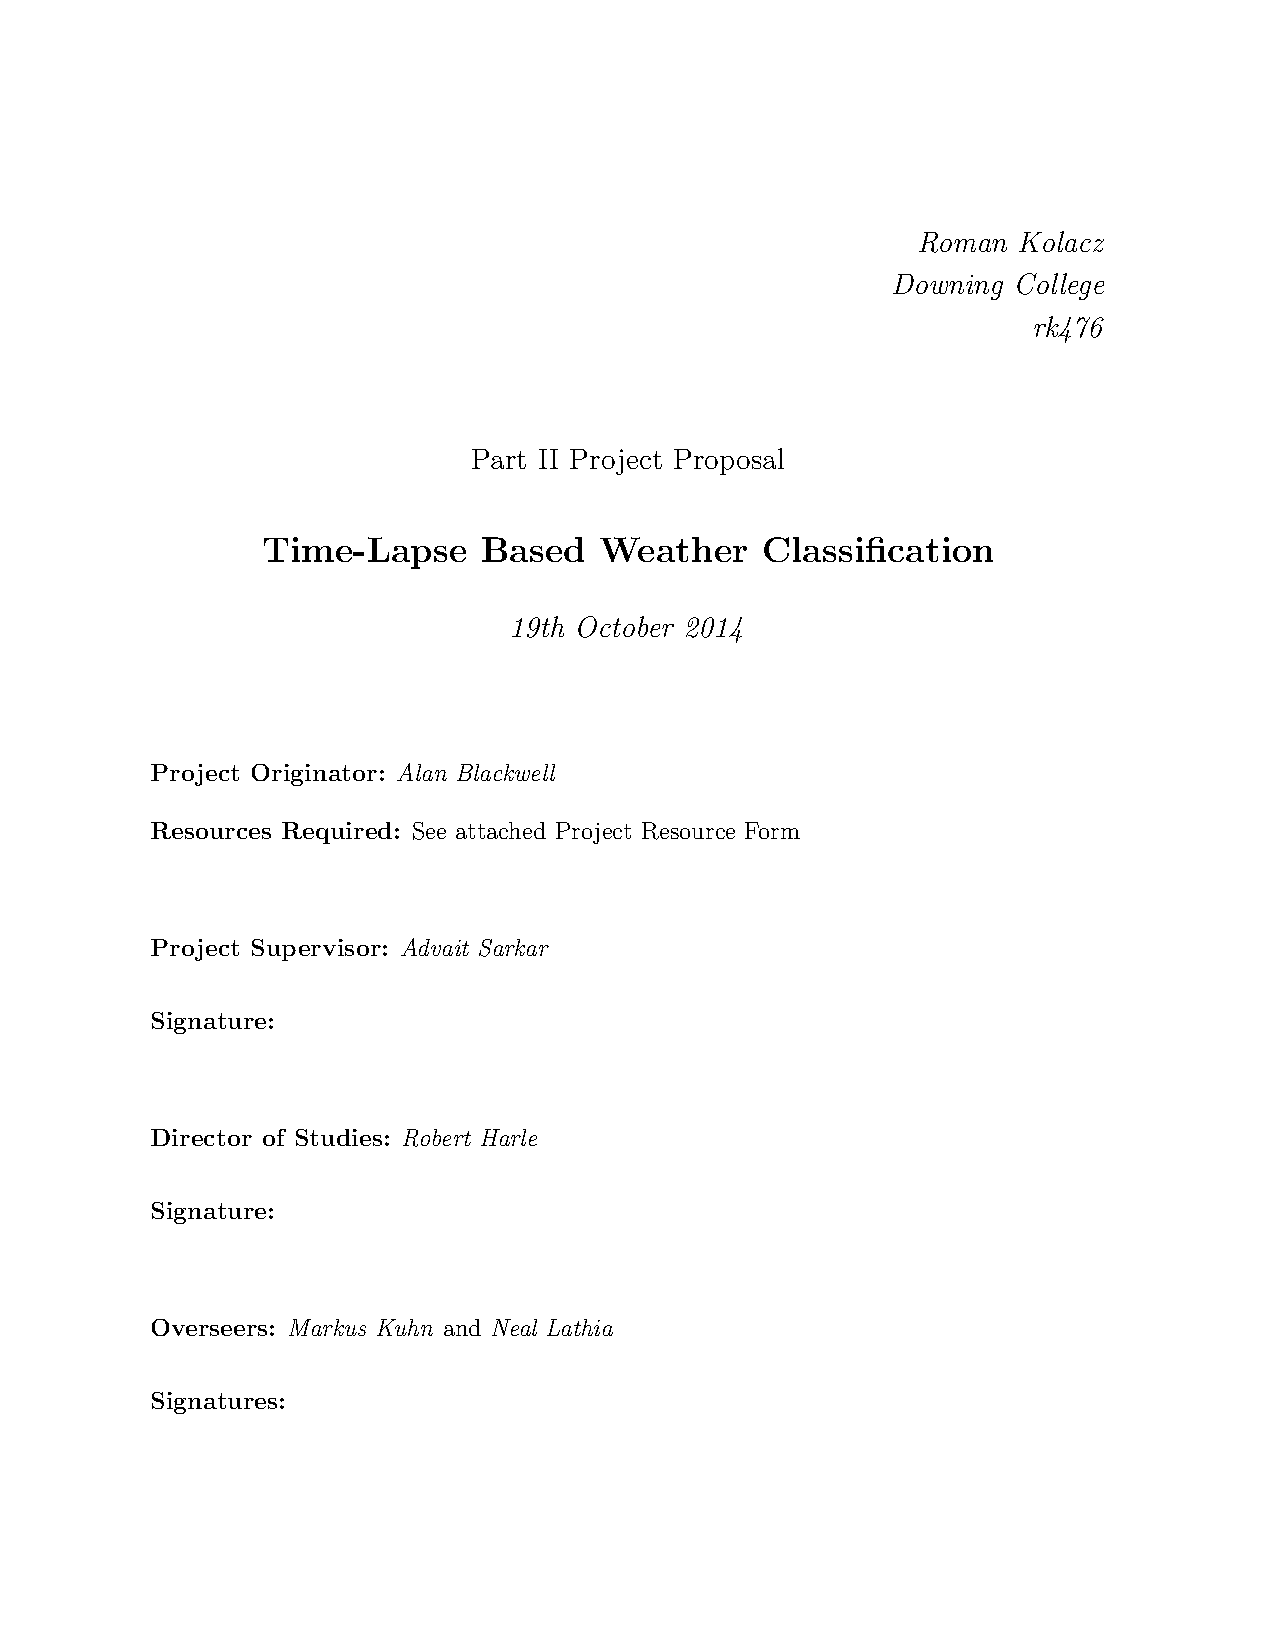
\includepdf[pages=-]{../projectplan/projectplan.pdf}

\end{document}

